\section{General idea of the backend sub-system}

\subsection{Hardware}
Before starting with the backend itself we need to describe the receiver and the antenna that is connected to the backend.


The ARTE project is intended to observe the milky way center, so we are in the case where we are observing a region that is fully populated with material affecting the DMs values. Although when I was working at the project we did not make an estimate of the DMs values that can be detected and just stick to the limitations that the hardware gave us. 


The antenna was designed by Diego Gallardo and consits of a dual polarization antenna array with a beam pattern that match the shape of the milky way, as the figure \ref{fig:arte_beam} shows. The single element of this array is based in two orthogonal microstrip dipoles (one for the x polarization and one for the y polarization) that can be seen in the figure \ref{fig:arte_element}.


You can look for more specification of the anntena \href{http://www.das.uchile.cl/lab_mwl/publicaciones/Articles/gallardo-et-al-2024-an-ultra-wideband-dual-polarization-antenna-array-for-the-detection-and-localization-of-bright-fast.pdf}{here}.

\begin{figure}
    \centering
    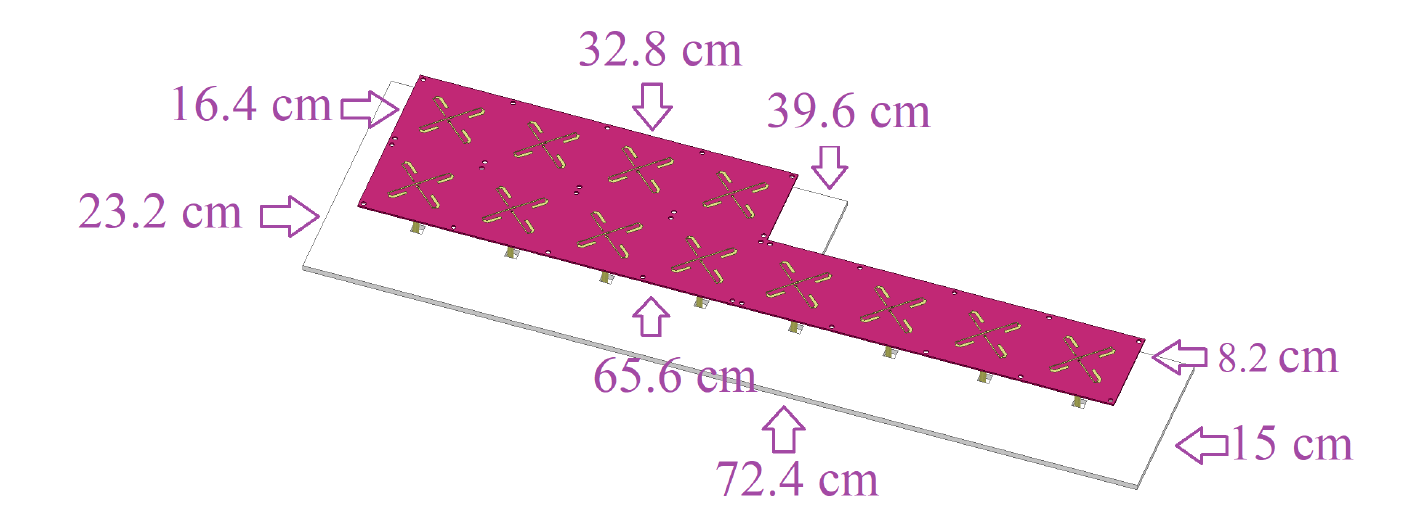
\includegraphics[width=0.7\textwidth]{images/arte_antenna.png}
    \caption{ARTE antenna diagram.}
    \label{fig:arte_array}
\end{figure}


\begin{figure}
    \centering
    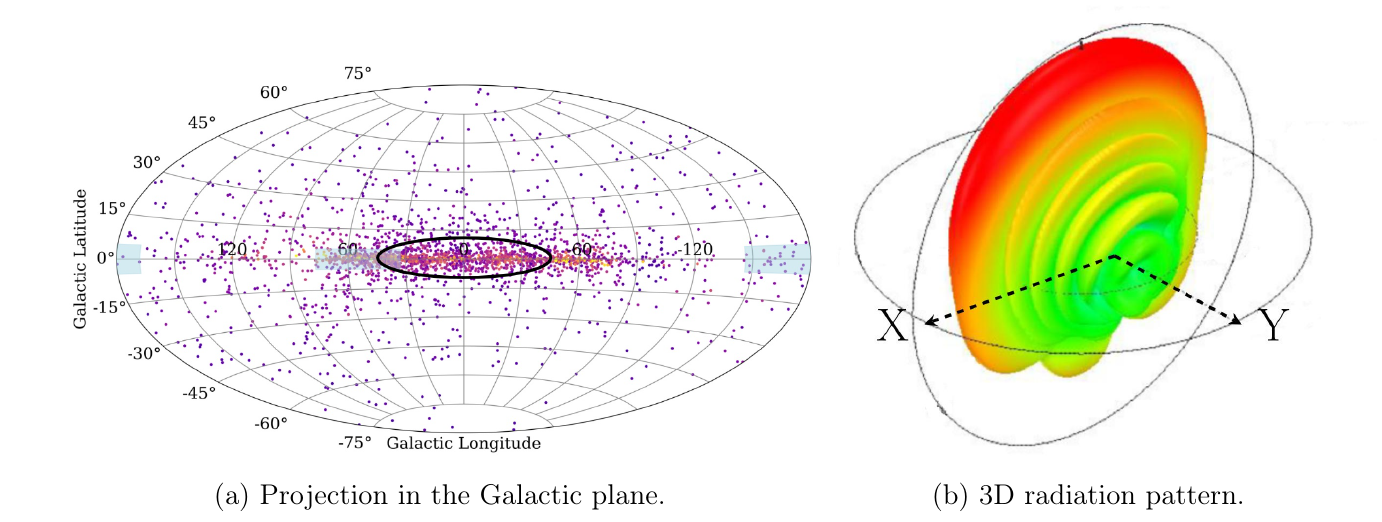
\includegraphics[width=0.7\textwidth]{images/arte_beam.png}
    \caption{ARTE simulated beam pattern and its projection over the milky way center..}
    \label{fig:arte_beam}
\end{figure}


\begin{figure}
    \centering
    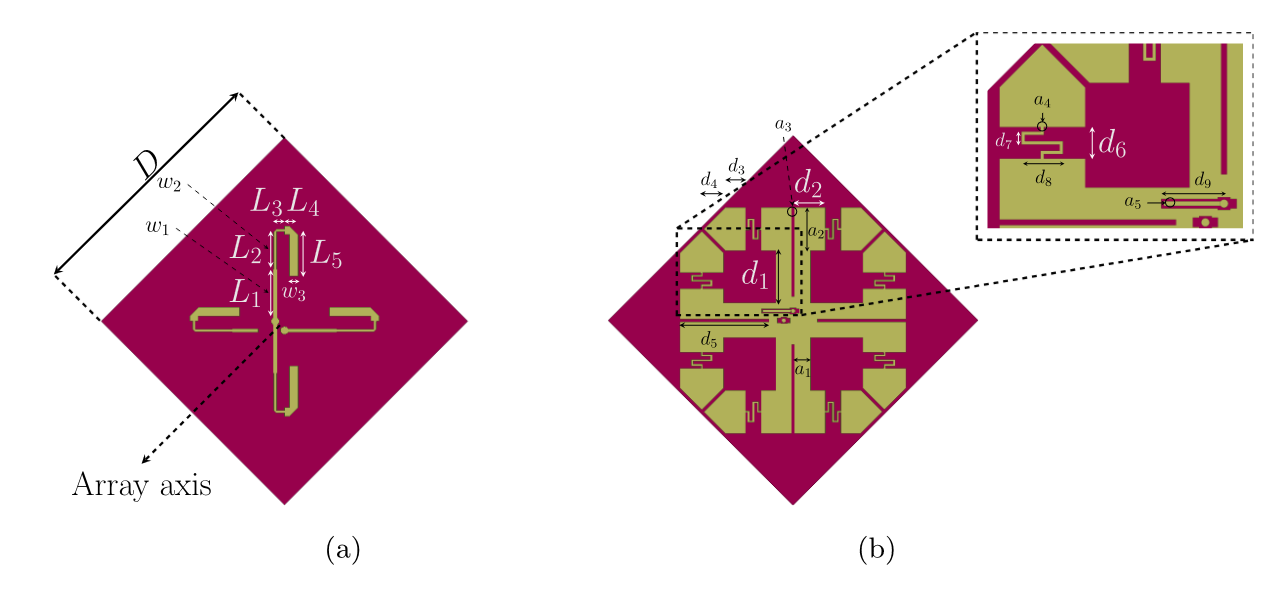
\includegraphics[width=0.7\textwidth]{images/arte_antenna_element.png}
    \caption{ARTE single element antenna.}
    \label{fig:arte_element}
\end{figure}




The receiver was built by Maximiliano Prieto and improved by Francisca Solis (you can take a look at their thesis for a technical description at the \href{http://www.das.uchile.cl/lab_mwl/publications.html}{mwl webpage}). For this document we only refer to the some key points:
\begin{itemize}
    \item The receiver bandwidth is $(1200-1800)$MHz. The bandwidth decision was made mainly for two reasons (if I recall correctly):
    \begin{enumerate}
        \item The digitizer that we have allows to see this band without any need of a downconvertion stage, so we would need only to filter out the undesired bands and put enough amplification to be able to observe.
        \item Looking at the chilean telecomunication regulation it has a good portion that is only for scientific usage.\footnote{Now I cant find the url but there is a huge document in the Subsecretaria de Telecomunicaciones regarding the RF spectrum usage.}.
    \end{enumerate}
        Now, when we started to comission this system we discover that the band was not as clean as we would like. In the figure \ref{fig:arte_rfi_meas} a RFI campaign and the bands usage is shown, it is worth to say that this capaign was a preliminar one and Francisca's thesis has way more werid detections.
    \begin{figure}
        \centering
        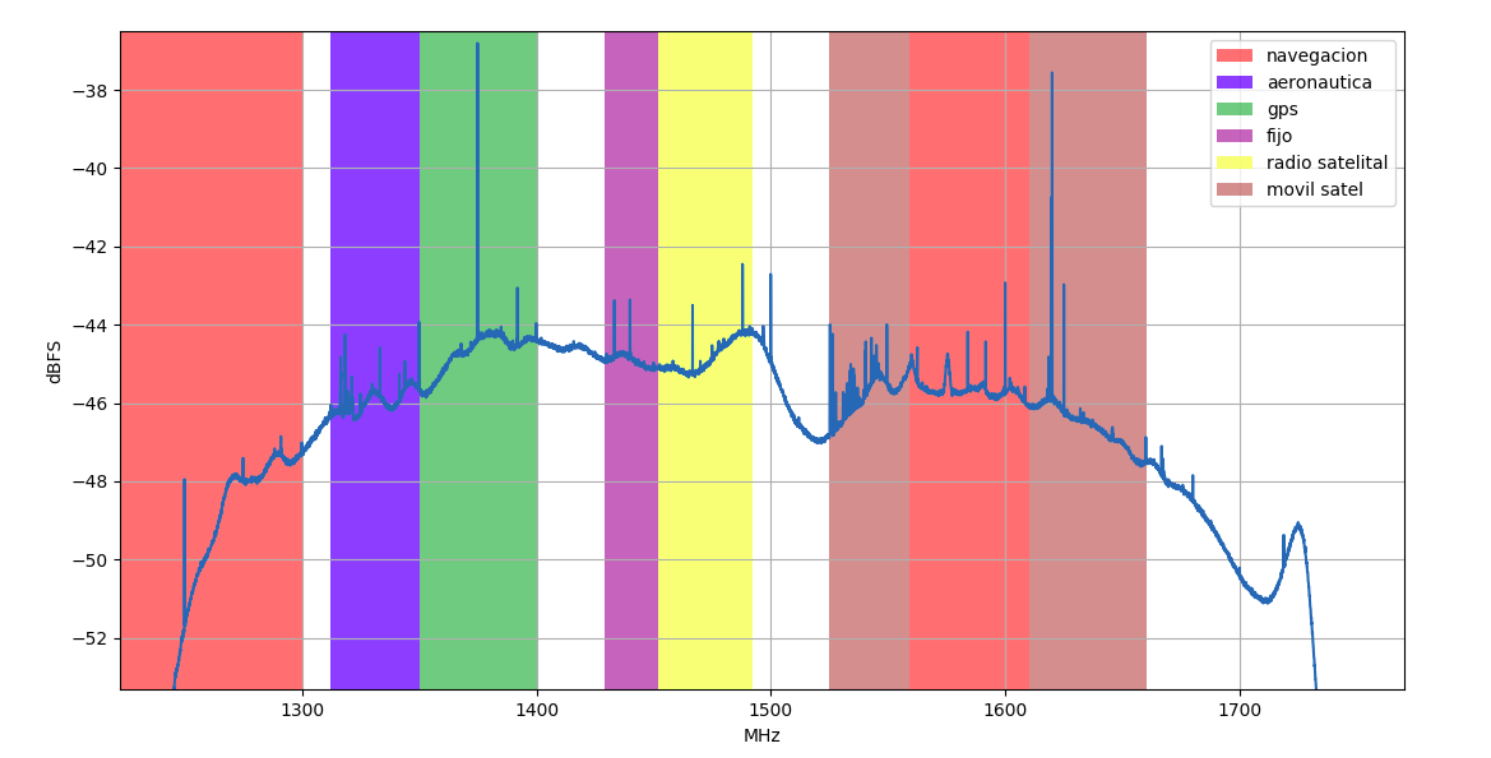
\includegraphics[width=0.7\textwidth]{images/arte_rfi_meas.png}
        \caption{Preliminar ARTE site RFI measurement at Cerro Calan and the bands usage by the SUBTEL.}
        \label{fig:arte_rfi_meas}
    \end{figure}

        To delimite the noise introduced by the adjacent bands the reciever has a pass-band filter at the desired frequency. But it is always good to keep in the back of your mind that can be that some images signals can pass by due the high gain of the receiver (although should be quite unusual..). Another thing that we discover in the comissioning stage is that the filters radiates the power and they can be capted by the antenna, so the shielding of the recevier has to be really good.
    
    \item The gain of the receiver is aorund 90dB (but dont belive me with eyes closed, I left the project some time ago and dont know what is the current status). There is a caveat here, as the antennas were in the top of the building and the receiver at the floor height there was a long cable that causes that system temperature were super high. As the noise equation says the first element its the one that influences the most, then the cables were ruining the sensitivity. Then, a set of low noise amplifiers was placed at the back-plane of the antennas to avoid having the long cables as first element.

    \item The amplifiers commonly have variations in gain, that gaves problems when trying to have an absolute measurement. A standard method is to place a load with known temperatures to calibrate the system. In the ARTE setup the hot load is a noise source that can be conneceted directly to the receiver via  a RF-switch that can be controlled to select between the antennas and this hot load.  Then you should have three temperatures available: The switch pointing to the antennas and having the measurement of the sky, the switch pointing to noise source in OFF status and the switch pointing to the noise source in ON status, then you can solve the equation to get the power-temperature conversion factor.
        It is worth to say that this is method just gave the receiver temperature, and disregard the antenna temperature measurement (a measurement that consider that should be way more complicated and I dont think that you would win too much with it, but is good to be aware of that).

        In the comissioning stage we discover that the gain fluctuates a lot, so we have to be constantly calibrating like every 5 or 10 minutes (again dont trust my numbers here).
    If you want more info about this read Francisca's thesis.
\end{itemize}

Ok, with this information we can finally start with the backend description, Yay!

\subsection{Backend system general idea}
As previously mentioned the selected bandwidth of the revceiver is in the (1200-1800)MHz range. To not use a downconversion scheme we decide to set the sample rate of the ADCs at 1.2GHz, giving us a baseband bandwidth of 600MHz, then the desired band should be in the third nyquist zone, using the \href{https://en.wikipedia.org/wiki/Undersampling}{undersampling} technique.
The undersampling technique is based in the use at your favor the aliasing effect. When an ADC is sampling at a given frequency $f_s$ the analog spectrum is divided in several zones that are multiple of $f_s/2$ as the figure \ref{fig:undersampling} shows. When passing from the analog to the digital realm all this zones are folded into the baseband, so you will have mixed the information of all the zones in the baseband and in principle you cannot separate them. Then, the trick for the undersample is just to filter out all the other zones that you are not interested in and use the aliasing folding mechanism to get the signal without a downconvertion.

The risk of using the undersampling technique is that you need to isolate the nyquist zone that you want to observe, otherwise undesired signals will leak into the baseband. For the ARTE case this was handled in the design of the receiver.

\begin{figure}
    \centering
    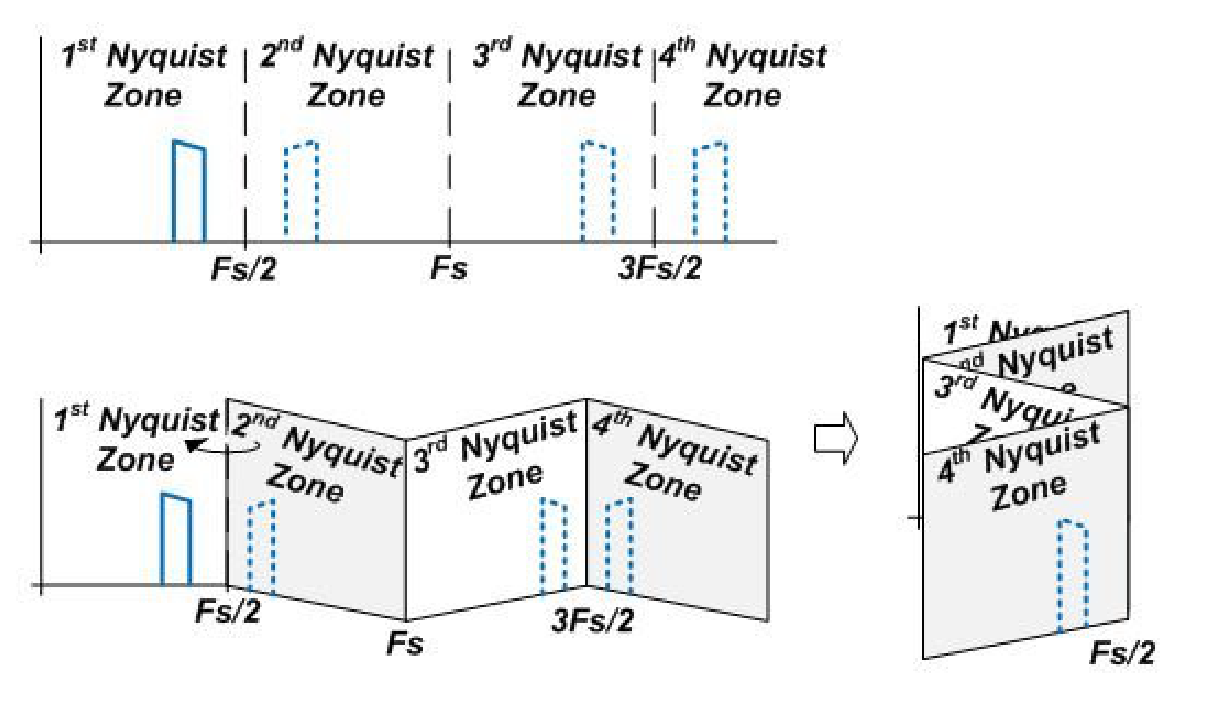
\includegraphics[width=0.7\textwidth]{images/undersampling.png}
    \caption{This figure shows the differnt nyquist zones that are defined by the ADC sampling frequency $f_s$. Note that the baseband has the information of all the nyquist zones, then to isolate one certain zone you need to us a bandpass filter.}
    \label{fig:undersampling}
\end{figure}


For the ARTE project was decided that we would use 4 ADCs: 3 used to digitize 3 sub-arrays of Diego's antennas and one antenna that will monitor the environment and flags detections as RFI when needed. The 4 ADCs have the same sampling frequency of 1.2GHz given by the same clock source.

When having the data digitized we have several subsystems that are running iside the FPGA. The figure \ref{fig:backend_diagram} shows the general diagram of the submodules that compose the backend system.
Here there is a little description of each submodule:
\begin{enumerate}
    \item The data temporal data of the 3 antennas that are looking at the sky is requantized from 8 bits to 4 bits and enters into a ring-buffer that is constantly writing the data in a circular way waiting for a signal that disable the write. This stop disable signal should be the detection of an astronomical transient event. To read the data from the ring-buffer we have a dedicated 1Gbe ethernet interface that is connected directly to the FPGA.
    \item Parallel to the ring-buffer saving, the 4 data stream from the ADCs passes through a polyphase filterbank structure and a Fast Fourier Transform to get the data in the frequency domain.
    \item The first two ADCs are complex added to get the elongated beam that should point to the center of the milky way.
    \item The beamformed spectra power is integrated a given time and is sent by one 10Gbe interface ot be offline processed. Some metadata should be in this packages, like for example the timestamp, status of the system, etc.
    \item In parallel, the 3 spectra that comes from Diego's antennas are used to compute the Direction of Arrival (DoA) of the sky signal. This was not implemented yet when I was in the project, but the main goal was to discard in real time signals that came from the horizon.
    \item With the beamformed signal and the spectra of the forth antenna we can use an RFI detection algorithm to rise a flag when there is RFI present and avoid having false detections.
    \item Since we found that there are some frequency channels that are constantly in use by human related task, we decided to flag some channels and set the power on them to zero.
    \item The flagged data enters into a incoherent dedispersion submodule, that is in charge of the real-time transient detection in the FPGA.
\end{enumerate}

In the following sections we will take a look to the different submodules and all the dirty tricks that I had to use to be able to compile the system.

\begin{figure}
    \centering
    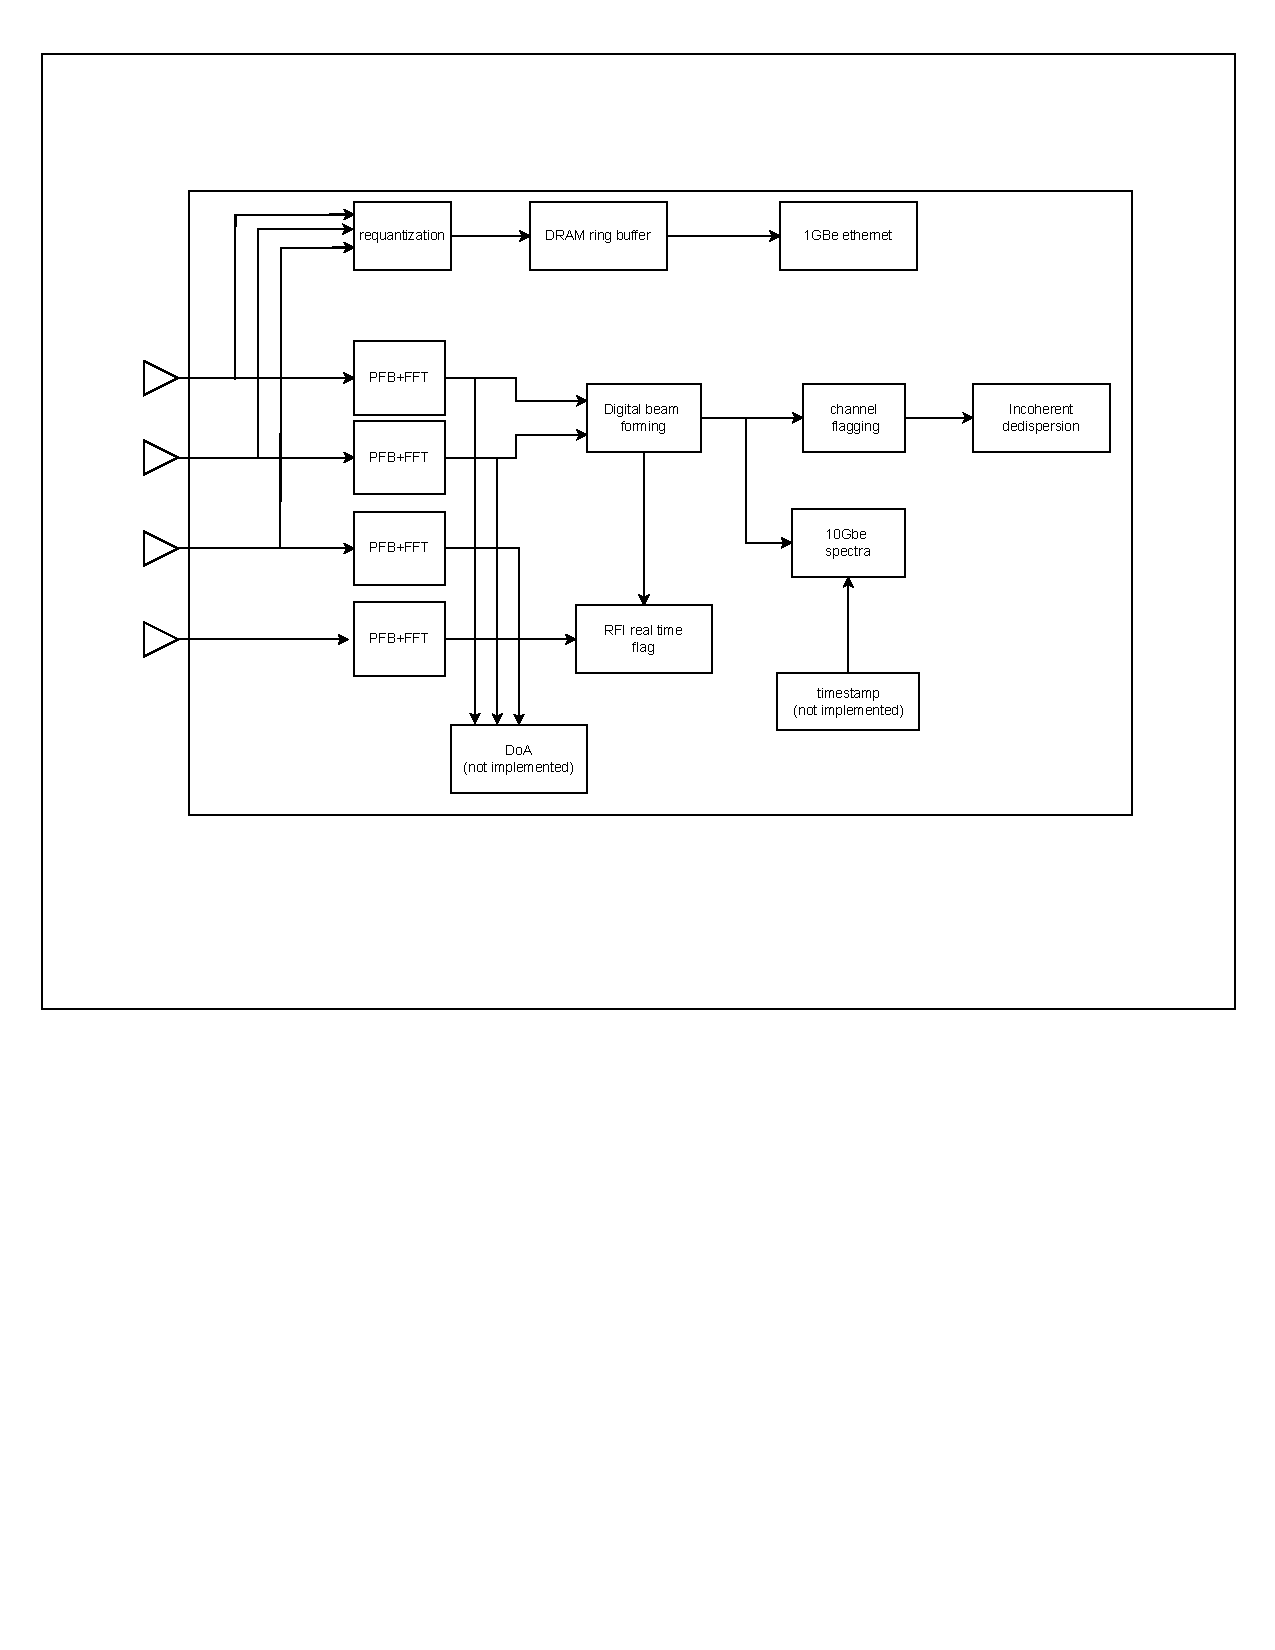
\includegraphics[width=\textwidth]{images/general_backend_diagram.pdf}
    \caption{This diagram shows the different subcomponents that are in the FPGA.}
    \label{fig:backend_diagram}
\end{figure}

\newpage
\subsection{ROACH2 presentation and installation hell}

The ARTE backend was designed in the ROACH2 platform that is a Virtex6 FPGA, connected to two 5GSa/s ADCs and to a PowerPC microprocessor. The Virtex6 family is an old FPGA family and then it is programmed using the old Xilinx ISE software, so you have to deal with a lot of deprecated information that is in the most hideous webpages. The ROACH2 platform is supported by the CASPER community that is an open source project that generate reusable cores for astronomical signal processing projects in a FPGA framework. That sounds awesome, until you discover that they fall in the trap of "simplify" the design process using simulink blocks. And as all the open source projects the documentation is almost non-existent\footnote{Similar to ARTE :p}.

The FPGA control is made by the PowerPC who has a direct bus connected to it. To handle request from the outside the PowerPC is runnning a server in the port 7147 where it accepts commands and translate it to FPGA register writing/reading. This is usually hide by the usage of a python package called \textbf{corr}. In addition the FPGA has a dedicated ethernet port that is directly connnected to the FPGA, and also you can connect 10Gbe interfaces. Having the network interfaces connected to the FPGA means that in its usage there is almost no software control involved and its controlled by digital logic (which makes TCP really complicated and we need to stick with UDP).




If you dont want to be overwhelmed with all the hussle of the software installation I strongly invite you to skip the following installation subsections and came back when you really need to do the installation in a fresh new computer.\footnote{I just want to state that I hate the toolflow as anyone else, and it was not my decision to make things that horrible.}

\subsubsection{FPGA toolflow installation}

\href{https://casper-toolflow.readthedocs.io/en/latest/src/Installing-the-Toolflow.html}{Here} you can find the installation requirements to install the ROACH2 toolflow. We found that is really a pain install everything since if you dont fulfill the requirements there is no garantee that you can install the software. The most notourius problem is regarding the OS, since having an ubuntu 14.04 has a lot of deprecated packages and you have to patch a lot of them\footnote{And the worst is that matlab and ISE use some OS packages instead of have their own!.}.
Because of that I started to use \href{https://wiki.archlinux.org/title/Systemd-nspawn}{nspawn} that can be used as a contained operative system, without having to emulate it. You just install a create a bunch of directories and then tell to the host operative system:"Hey, now instead of looking for a certain package in the root directory you will look it here".

I made some automatic scripts to install the complete toolflow in a consistent way and I had try it in different Debian based operative system. I left the installer in the digital backup hard drive and is called \textbf{"auto\_install\_casper\_roach"}. In this installation directory I left all the patched softwares and make the installation using Makefiles. A Makefile is just a set of instructions that the terminal will run when you gave the command \textbf{make <some\_insctruction>} \footnote{Even if you dont use the Makefile is a good way to store the commands that you would probably need when installing the toolflow manually}.


When runnign that successfully you will have a directory called \textbf{casper} in your home directory and inside you will have the complete ubuntu directory tree. In the \textbf{~/casper/home/Workspace/} you will have the \textbf{mlib\_devel} directory, where you can launch the casper toolflow. It is important to use the \textbf{mlib\_devel} version that is pointed in the Makefile, since it is a modified version that has a trick to use the DRAM in the ROACH2 (the oficial casper one do not let you use the DRAM module). 



The installer also should have create some alias to start the container just typing \textbf{boot-roach-env} and with that you will be in the container.
So as a summary, to start the container just type \textbf{boot-roach-env}, if you want to have more than one instance then you need to use the \textbf{machinectl login casper} command. To shut it down just type \textbf{poweroff} on one of the containers terminals.

To run the toolflow you just need to go the \textbf{/home/Workspace/mlib\_devel} and run the \textbf{./startsg} file, it will start matlab with all the dependencies and with that you can finally start to design the models for your FPGA.





\subsubsection{More dependencies and installations}
The previous section explained how to get the software to program the FPGA, but thats only one portion of the programming scheme, you need a way to communicate with the FPGA. The communication with the FPGA is done by the PowerPC that has a direct connection with it via a digital bus called OPB that was an IBM standard to communicate chips. 
The RAOCH2 PowerPC has a linux OS called BORPH that runs a telnet server in the port 7147 where you can send commands in the KATCP standard. Among these commads there are some write/read commmands that you can use to interrogate the FPGA from the PowerPC and sent the answer back to the client computer. 
\href{https://casper.berkeley.edu/wiki/Tcpborphserver}{here} you have a description of the protocol and the common commands.

To make things a little bit easier the casper people create the \textbf{corr} python package that use the KATCP protocol under the hood for us. But as always, this has to be painfull and it only works with python2.7 that is fully deprecated. 
The way to go is either use the container created previously or create your own with Docker or something like that,

If the number of abstractions dont make you mad yet, we created another python package in top of corr to handle typical actions for the FPGA programming. You can find my modified package \href{https://github.com/sebajor/calandigital}{here} and you should be able to install all the dependencies with pip in the container.


\subsubsection{ARTE control codes}
For the ARTE project we created a special repository called \textbf{ARTE-control} that you could get \href{https://github.com/sebajor/ARTE-control/}{here}. It have a requirements file to install with pip. 

This repository will be described later, after the explanation of the FPGA program side, because it interacts directly with it. The only things to note now are:
\begin{itemize}
    \item There is a configuration file that contains the hyperparameters of the system.
    \item With the \textbf{init.py} code you initialize and configure the FPGA.
    \item The codes directory contains all the control codes and the real time ploting codes. If you want to interface with the FPGA by yourself most of the functions are in \textbf{codes/utils}.
    \item In the codes directory there is a \textbf{logger.py} script that collects data from the 10Gbe interface.
    \item The postprocessing directory has some codes to plot collected data from the 10Gbe interface.
    \item There is a \textbf{debug\_codes} directory that contains models that are not limited by the resource usage of the main ARTE model. They can be used to be sure that some measurements values are not created by the digital truncation of the main model.
\end{itemize}



\subsubsection{ROACH2 DRAM kernel}
To keep doing this more complicated, the default kernel that cames with the ROACH2 is not compatible with the usage of the DRAM so you need to pass a modified one. This can be done when the system is booting, stoping the boot process and sending the kernel, uboot and the linux image via a tftp server. Be super carefull when doing this and test that the tftp is really working, otherwise you could erase the booting memory and then you will need to do \href{https://www.mail-archive.com/casper@lists.berkeley.edu/msg08171.html}{some black magic} to get them back.

\href{https://github.com/sebajor/simulink_models/tree/master/DRAM/ROACH2}{Here} you have some instructions of what to do. I hope you do not have to do this, because is super obscure and I left at least 2 ROACH with this kernel version.

You can see that the ROACH2 does not have the right kernel if when uploading the bof file the system will complain about a non-responding model or something like that.


\subsubsection{Installation summary}
At the end you should have access to the following softwares/packages:
\begin{itemize}
    \item ISE, Matlab and the \textbf{mlib\_devel} with all the needed patches (you should be able to compile a test model). Optionally you can have the nspawn container.
    \item \textbf{calan\_digital} with all its dependencies.
    \item ARTE control with all its depencies
    \item A ROACH2 with the modified kernel. If you dont have the modified one the system initialization of the bit file will fail.
\end{itemize}



